\newpage
\subsection{UC4 - Creazione di un grafico}
\label{sub:uc2}

\begin{figure}[h]
    \centering
    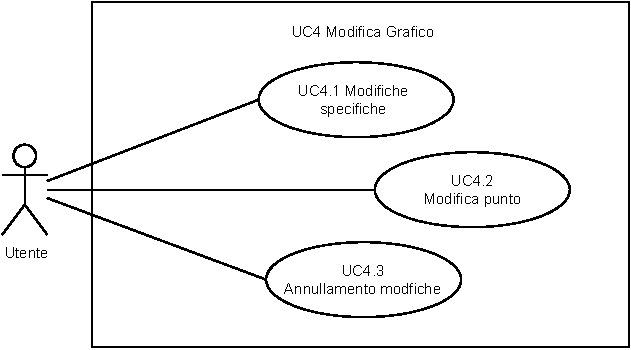
\includegraphics[width=0.5\textwidth]{componenti/casi-duso/diagrammi/UC4.pdf}
    \caption{Diagramma rappresentante UC4}
    \label{fig:UC2}
\end{figure}


\begin{itemize}
    \item \textbf{Descrizione}: L’utente vuole procedere con la fase di esplorazione
                                dati mediante la visualizzazione del dataset
                                attraverso uno dei diversi grafici proposti dall’applicativo
                                che ne costruisce uno e lo visualizza.
	
    \item \textbf{Attore primario}: Utente;
    
    \item \textbf{Precondizione}:   Nel progetto corrente è stato importato un dataset e ogni 
                                    suo campo ha un metatag associato;

    \item \textbf{Postcondizione}:  Viene calcolato il grafico della tipologia scelta dai dati del progetto 
                                    corrente e visualizzato
	\item \textbf{Scenario principale}:
		\begin{enumerate}
			\item L'utente seleziona la tipolgoia di grafico che vuole creare (UC4.1);
			\item HDviz visualizza il grafico ottenuto dalla costruzione dei dati (UC5);
        \end{enumerate}

    \item \textbf{Inclusioni}: 
            \begin{itemize}
                \item UC10: Visualizazzione di un grafico.
            \end{itemize}
    \end{itemize}


\subsection{UC4.1 - Selezione di un grafico}

\begin{itemize}
    \item \textbf{Descrizione}: L’utente vuole procedere con la fase di esplorazione
                                dati mediante la visualizzazione del dataset
                                attraverso uno dei diversi grafici proposti dall’applicativo
                                che ne costruisce uno.
	
    \item \textbf{Attore primario}: Utente;
    
    \item \textbf{Precondizione}:   Un dataset è stato correttamente importato e ad ogni campo ha associato
                                    un metatag;

    \item \textbf{Postcondizione}:  Viene calcolato il grafico della tipologia scelta dai dati del progetto 
                                    corrente
	\item \textbf{Scenario principale}:
		\begin{enumerate}
			\item L'utente seleziona la tipolgoia di grafico che vuole creare;
        \end{enumerate}
    \item \textbf{Generalizzazioni:}:  L'utente seleziona il grafico desiderato:
        \begin{itemize}
            
            \item Grafico scatterplot matrix (UC4.1a).
            \item Grafico force field (UC4.1b).
            \item Grafico heat map (UC4.1c).
            \item Grafico proiezione lineare multiasse (UC4.1d).
            
        \end{itemize}
    
    \item \textbf{Inclusioni}: 
            \begin{itemize}
                \item UC10: Visualizazzione di un grafico.
            \end{itemize}
    \end{itemize}

\subsection{UC4.1.a Selezione di Scatterplot matrix}

\begin{itemize}

    \item \textbf{Attore primario}: Utente;

    \item \textbf{Precondizione}:   Un dataset è stato correttamente importato e ad ogni campo ha associato
                                    un metatag;

    \item \textbf{Postcondizione}:  Viene calcolato il grafico di tipo Scatterplot matrix dal progetto corrente
  
\end{itemize}


\subsection{UC4.1.b Selezione di Force Field}

\begin{itemize}

    \item \textbf{Attore primario}: Utente;

    \item \textbf{Precondizione}:   Un dataset è stato correttamente importato e ad ogni campo ha associato
                                    un metatag;

    \item \textbf{Postcondizione}:  Viene calcolato il grafico di tipo Force Field dal progetto corrente
  
\end{itemize}


\subsection{UC4.1.c Selezione di Heat Map}

\begin{itemize}

    \item \textbf{Attore primario}: Utente;

    \item \textbf{Precondizione}:   Un dataset è stato correttamente importato e ad ogni campo ha associato
                                    un metatag;

    \item \textbf{Postcondizione}:  Viene calcolato il grafico di tipo Heat map dal progetto corrente
  
\end{itemize}


\subsection{UC4.1.d Selezione di Proiezione lineare multiasse}

\begin{itemize}

    \item \textbf{Attore primario}: Utente;

    \item \textbf{Precondizione}:   Un dataset è stato correttamente importato e ad ogni campo ha associato
                                    un metatag;

    \item \textbf{Postcondizione}:  Viene calcolato il grafico di tipo \emph{"Proiezione lineare multiasse"} dal progetto corrente
  
\end{itemize}


